\chapter{Resultados Preliminares}

Neste capítulo será apresentado os resultados premliminares, onde utilizamos o diagrama de caso de uso apresentado na Figura \ref{figura:sistemadicas} encontrada no Capítulo 3 para realizar o desenvolvimento do sistema no \foreign{framework} de desenvolvimento Laravel na versão 5.1.

Assim foi desenvolvido o registro de usuário, o login, a tela de resetar senha, o cadastro de professor e o cadastro de aluno representadas respectivamente nas figuras a seguir.

\begin{figure}[]
	\captionsetup{justification=centering}
	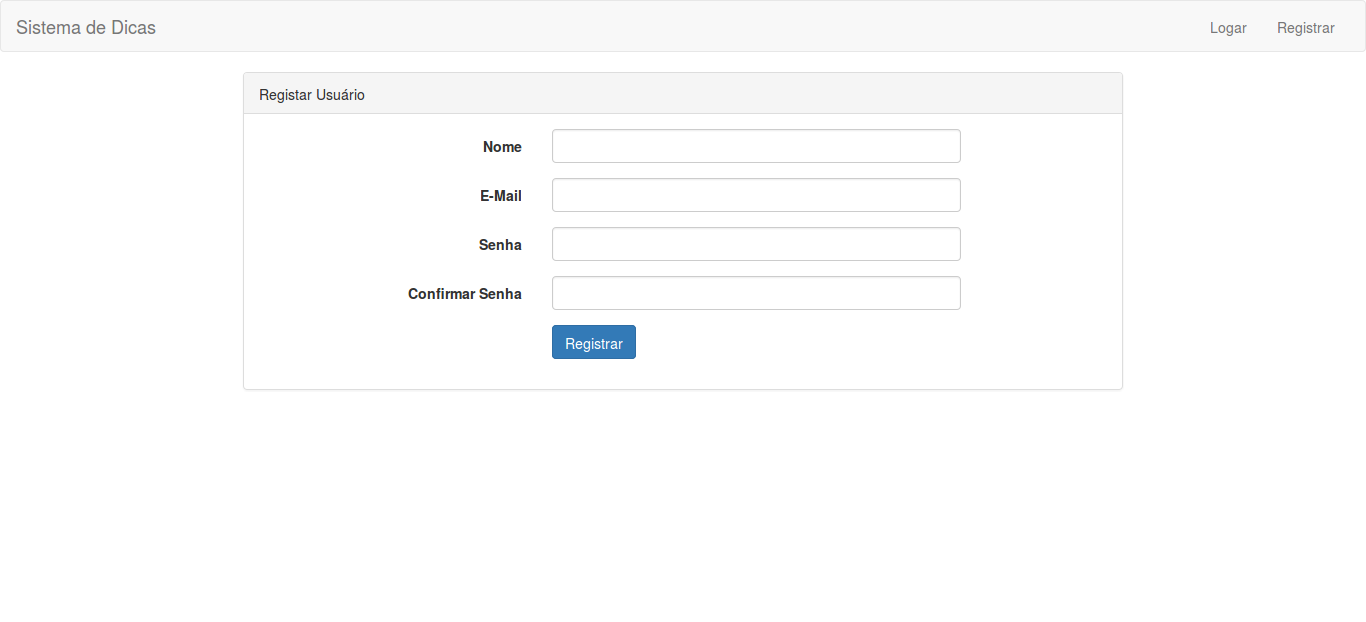
\includegraphics[width=\linewidth]{imagenssoftware/registrarusuario.png}
	\caption{Tela de regustro de usuário.}
	\label{figura:registrarusuario}
\end{figure}

\begin{figure}[h]
	\captionsetup{justification=centering}
	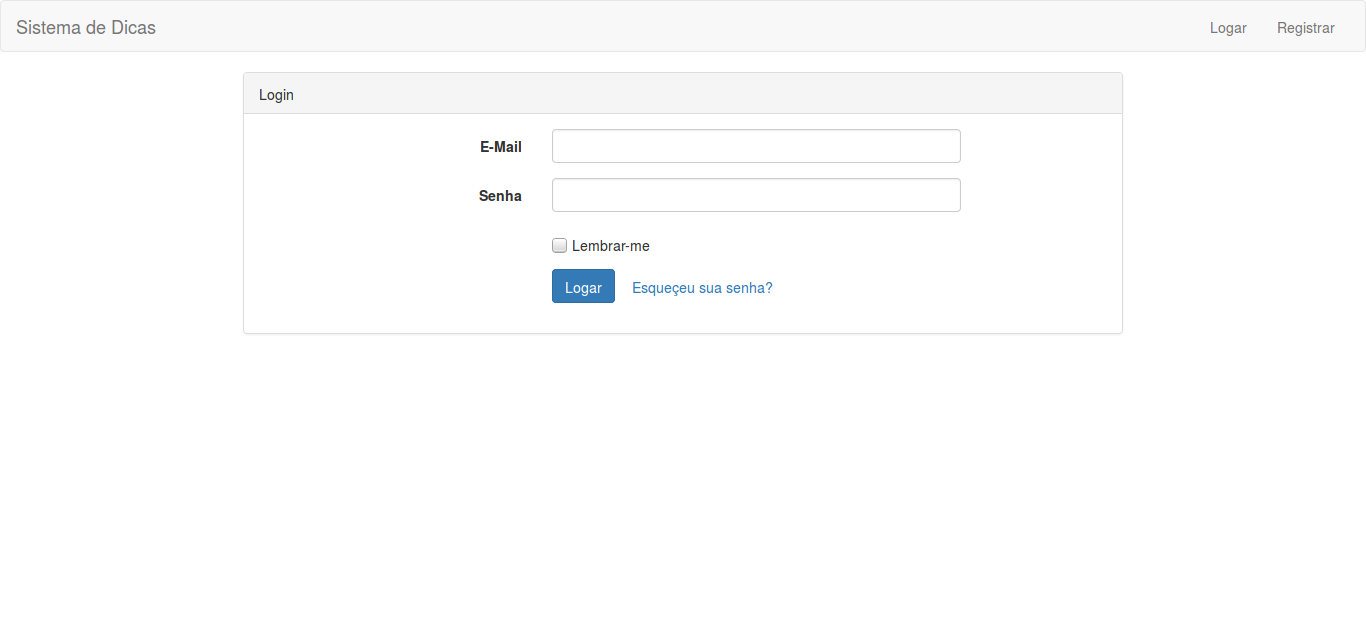
\includegraphics[width=\linewidth]{imagenssoftware/logar.png}
	\caption{Tela de login no sistema.}
	\label{figura:logar}
\end{figure}

\begin{figure}[h]
	\captionsetup{justification=centering}
	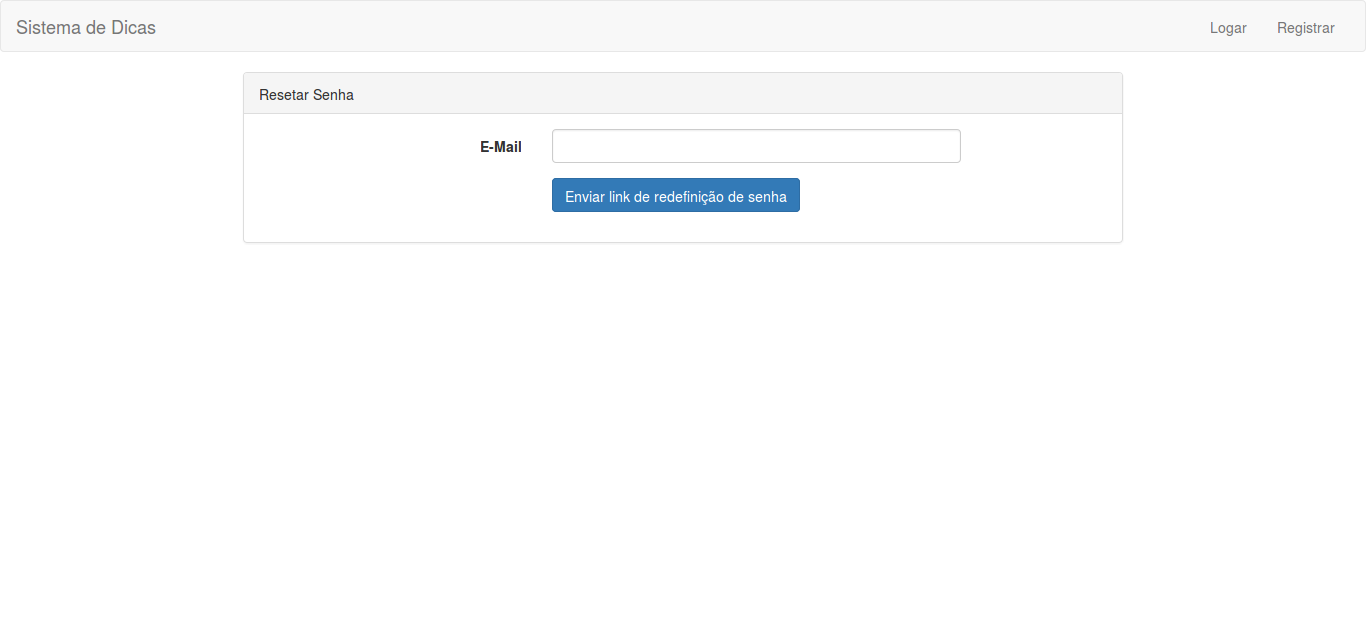
\includegraphics[width=\linewidth]{imagenssoftware/resetarsenha.png}
	\caption{Tela para resetar a senha.}
	\label{figura:resetarsenha}
\end{figure}

\begin{figure}[h]
	\captionsetup{justification=centering}
	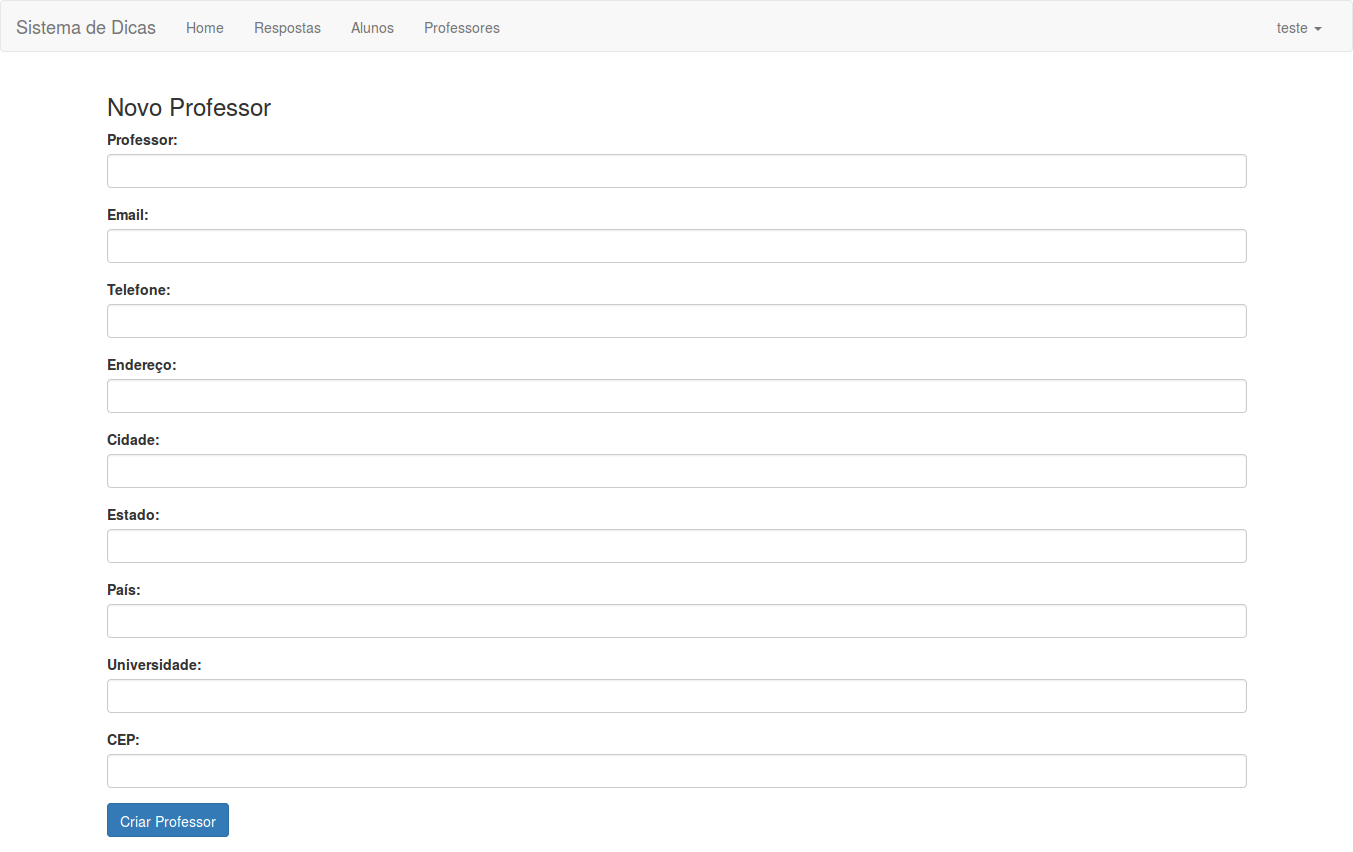
\includegraphics[width=\linewidth]{imagenssoftware/cadastroprofessor.png}
	\caption{Tela de cadastro de professor.}
	\label{figura:cadastroprofessor}
\end{figure}

\begin{figure}[h]
	\captionsetup{justification=centering}
	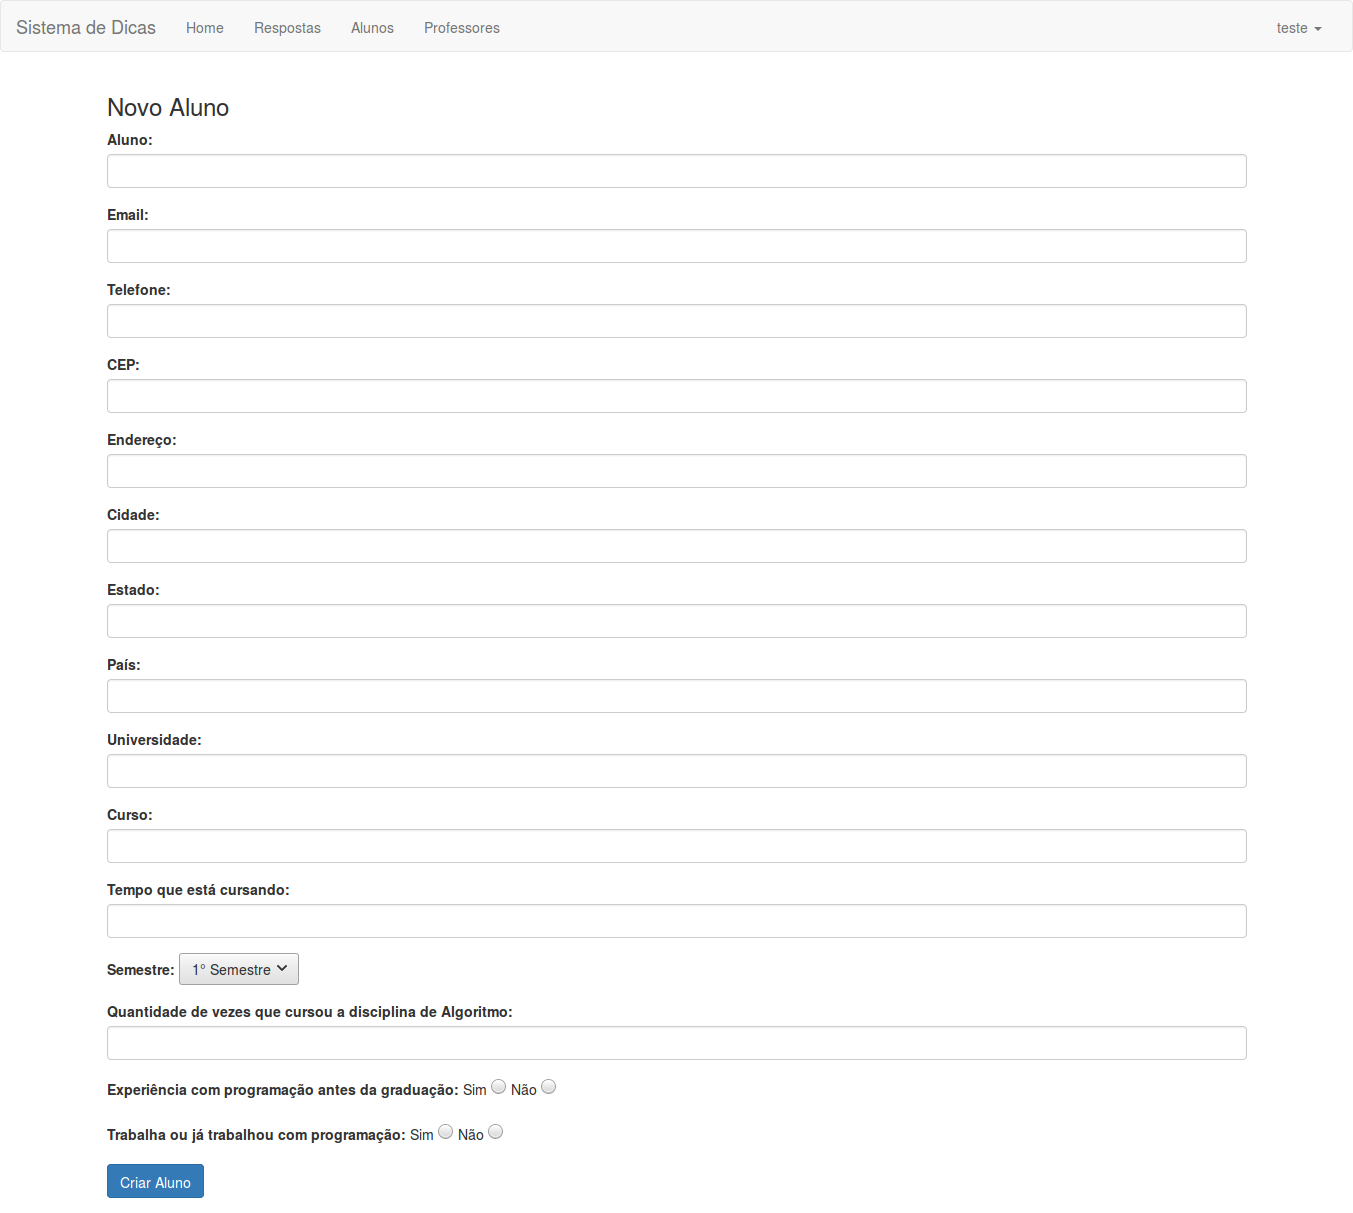
\includegraphics[width=\linewidth]{imagenssoftware/cadastroaluno.png}
	\caption{Tela de cadastro de aluno.}
	\label{figura:cadastroaluno}
\end{figure}